%% start of file `template.tex'.
%% Copyright 2006-2015 Xavier Danaux (xdanaux@gmail.com).
%
% This work may be distributed and/or modified under the
% conditions of the LaTeX Project Public License version 1.3c,
% available at http://www.latex-project.org/lppl/.


\documentclass[11pt,a4paper,sans]{moderncv}        % possible options include font size ('10pt', '11pt' and '12pt'), paper size ('a4paper', 'letterpaper', 'a5paper', 'legalpaper', 'executivepaper' and 'landscape') and font family ('sans' and 'roman')
\usepackage{ragged2e}
\usepackage{lastpage}

\usepackage{fancyhdr}

\fancyfoot[C]{ \thepage\ / \pageref{LastPage}}
\usepackage{pdfpages}
% moderncv themes
\moderncvstyle{casual}                             % style options are 'casual' (default), 'classic', 'banking', 'oldstyle' and 'fancy'
\moderncvcolor{blue}                               % color options 'black', 'blue' (default), 'burgundy', 'green', 'grey', 'orange', 'purple' and 'red'
%\renewcommand{\familydefault}{\sfdefault}         % to set the default font; use '\sfdefault' for the default sans serif font, '\rmdefault' for the default roman one, or any tex font name
%\nopagenumbers{}                                  % uncomment to suppress automatic page numbering for CVs longer than one page

% character encoding
%\usepackage[utf8]{inputenc}                       % if you are not using xelatex ou lualatex, replace by the encoding you are using
%\usepackage{CJKutf8}                              % if you need to use CJK to typeset your resume in Chinese, Japanese or Korean

% adjust the page margins
\usepackage[scale=0.75]{geometry}
%\setlength{\hintscolumnwidth}{3cm}                % if you want to change the width of the column with the dates
%\setlength{\makecvtitlenamewidth}{10cm}           % for the 'classic' style, if you want to force the width allocated to your name and avoid line breaks. be careful though, the length is normally calculated to avoid any overlap with your personal info; use this at your own typographical risks...

% personal data
\name{Fabian E.}{Gruber}
%\title{Resumé title}                               % optional, remove / comment the line if not wanted
\address{Anna-Stainer-Knittel-Weg 3/5/4}{6020 Innsbruck, Austria}% optional, remove / comment the line if not wanted; the "postcode city" and "country" arguments can be omitted or provided empty
\phone[mobile]{+43~650~2587521}                   % optional, remove / comment the line if not wanted; the optional "type" of the phone can be "mobile" (default), "fixed" or "fax"
%\phone[fixed]{+2~(345)~678~901}
%\phone[fax]{+3~(456)~789~012}
\email{Fabian.Gruber@uibk.ac.at}                               % optional, remove / comment the line if not wanted
%\homepage{www.johndoe.com}                         % optional, remove / comment the line if not wanted
%\social[linkedin]{john.doe}                        % optional, remove / comment the line if not wanted
%\social[twitter]{jdoe}                             % optional, remove / comment the line if not wanted
%\social[github]{jdoe}                              % optional, remove / comment the line if not wanted
%\extrainfo{additional information}                 % optional, remove / comment the line if not wanted
\photo[64pt][0.2pt]{IMG_3890_cropped2}                       % optional, remove / comment the line if not wanted; '64pt' is the height the picture must be resized to, 0.4pt is the thickness of the frame around it (put it to 0pt for no frame) and 'picture' is the name of the picture file
%\quote{}                                 % optional, remove / comment the line if not wanted

% bibliography adjustements (only useful if you make citations in your resume, or print a list of publications using BibTeX)
%   to show numerical labels in the bibliography (default is to show no labels)
\makeatletter\renewcommand*{\bibliographyitemlabel}{\@biblabel{\arabic{enumiv}}}\makeatother
%   to redefine the bibliography heading string ("Publications")
%\renewcommand{\refname}{Articles}

% bibliography with mutiple entries
%\usepackage{multibib}
%\newcites{book,misc}{{Books},{Others}}
%----------------------------------------------------------------------------------
%            content
%----------------------------------------------------------------------------------
\begin{document}
%\begin{CJK*}{UTF8}{gbsn}                          % to typeset your resume in Chinese using CJK

%-----       letter       ---------------------------------------------------------
% recipient data
\recipient{SynerGIS Informationssysteme GmbH \\z.H. Herrn Gernot Tutsch}{Technologiestra{\ss}e 10\\1120 Wien}
\date{15. Dezember, 2018}
\opening{Sehr geehrter Herr Tutsch,}
\closing{Mit besten Gr\"{u}{\ss}en,}
\enclosure[Anhang]{Lebenslauf, Publikationsliste und Diplombescheid}       % use an optional argument to use a string other than "Enclosure", or redefine \enclname

\makelettertitle
\justify
Hiermit m\"ochte ich mich f\"ur die Stelle des GIS Team Mitarbeiters bewerben. Zur Zeit bin ich noch als wissenschaftlicher Mitarbeiter an der LFU Innsbruck am Institut f\"ur Geographie angestellt und schreibe an meiner Dissertation mit dem Titel 'Digital terrain analysis to support field soil survey'.

Erste Erfahrungen mit GIS machte ich bereits im Rahmen meines Studiums der Kulturtechnik und Wasserwirtschaft an der Universit\"at f\"ur Bodenkultur (Wien), wo ich  den vertiefenden Wahlfachblock 'Photogrammetrie und Fernerkundung'  absolvierte, der auch eines meiner beiden Diplompr\"ufungsf\"acher darstellte. Als studentischer Mitarbeiter am Institut f\"ur Angewandte Geologie war ich an dem Projekt 'Remote Geohazards Assessment in Tajikistan (TajHaz)' beteiligt, bei dem mit GIS und Fernerkundungsmethoden ein Ereignis- und Seenkataster f\"ur abgelegene Regionen in Tajikistan erstellt wurde. Weiters war ich w\"ahrend meiner Studienzeit als ArcGIS-Tutor im Rahmen der Lehrveranstaltung 'Einf\"uhrung in GIS' angestellt. Nach meiner Diplomarbeit am Institut f\"ur Angewandte Geologie, welche sich mit der Modellierung von Bergsturzseeausbr\"uchen  besch\"aftigte, war ich weiterhin als Projektmitarbeiter an diesem Institut besch\"aftigt im Rahmen des Projekts 'Poverty Alleviation through Mitigation of Integrated High-Mountain Risk (PAMIR)'. Dabei wurden regionale Naturgefahrenhinweiskarten mithilfe einer Kombination aus automatisierter sowie expertenbasierter Kartierung und Klassifikation erstellt.

Im Sommer 2013 wechselte ich als Projektmitarbeiter ans Institut f\"ur Geographie in Innsbruck, wo  im Rahmen des Projekts 'Reliefklassifizierung aus ALS Daten als Grundlage f\"ur die Regionalisierung von Bodendaten (ReBo)' weiterhin die Arbeit mit Geoinformationssystemen zu meinen t\"aglichen Aufgaben geh\"orte, wobei hier haupts\"achlich quelloffene GIS, vor Allem GRASS GIS und Quantum GIS, aber auch SAGA GIS, verwendet wurden. Statistische Analysen der Geodaten, sowie darauf basierendes statistisches Lernen, wurden mit R, der freien Programmiersprache f\"{u}r statistisches Rechnen, durchgef\"uhrt. Python Scripts dienten zur Automatisierung von Rechenabl\"aufen in GRASS und SAGA GIS. In Innsbruck begann auch eine intensive Auseinandersetzung mit maschinellem Lernen, etwa zur r\"aumlichen Modellierung von Gel\"andeformen  oder dem Bodenausgangsmaterial f\"ur die Anwendung in der klassischen Bodenkartierung. 


Die intensive Besch\"aftigung mit Open Source Geoinformationssystemen hat mir, wenn auch nicht ArcGIS-spezifisch, wichtige Einblicke in die Funktionsweise von GIS im Allgemeinen, sowie darin integrierten  spezifischen Tools gebracht. Meine Python-Grundlagen erlauben mir neben der Automatisierung von Abl\"aufen zur L\"osung spezifischer, vor Allem raumbezogener, Aufgaben auch Einsicht in den Code vieler GIS-Tools zu nehmen und die tats\"achlichen Berechnungen besser zu verstehen. Aufgrund meiner langj\"{a}hrigen Erfahrung als Projektmitarbeiter an verschiedenen Universit\"{a}ten bringe ich viel Erfahrung in selbstst\"{a}ndiger Arbeit mit, genauso aber auch Erfahrung in der Zusammenarbeit mit Personen aus unterschiedlichen Fachgebieten. Meine Lernbereitschaft zeigt sich einerseits in der selbstst\"andigen Einarbeitung in neue Themen und Software im Rahmen meiner Forschungst\"atigkeiten, sowie andererseits in der freiwillige Teilnahme und  Absolvierierung von Onlinekursen wie z.B. 'Statistical learning' von Stanford Online oder 'Echoes in Space - Introduction to radar remote sensing' der ESA. Dies unterstreicht auch mein ausgepr\"agtes Interesse an Geoinformation und verwandten Bereichen. Die Arbeit als Lektor im Fach '\"Ubungen zur Statistik' zeigt wiederum mein Interesse daran, selbst angeeignetes Wissen weiter zu geben.

Nach mehren Jahren der T\"atigkeit an Universit\"aten m\"ochte ich nun ein neues Kapitel aufschlagen und mich f\"ur die ausgeschriebene Stelle bewerben. An der Stelle reizt mich sowohl die M\"oglichkeit mich auch in Zukunft intensiv mit GIS besch\"aftigen zu k\"onnen, als auch  Anwender bei der Analyse und L\"osung von Problemen zu unterst\"utzen . \"Uber eine Einladung zu einem Gespr\"ach w\"urde ich mich freuen.

\makeletterclosing
\clearpage
%-----       resume       ---------------------------------------------------------
\makecvtitle


\section{Berufserfahrung}
\cventry{2013--Heute   }{Wissenschaftlicher Mitarbeiter}{Institut f\"{u}r Geographie, Universit\"{a}t Innsbruck}{Innsbruck}{}{Forschungsprojekte: 
\begin{itemize}%
\item Shallow erosion dynamics in mountain grasslands of South Tyrol: Monitoring, process analysis and mitigation measures (EroDyn)
  \begin{itemize}%
  \item Geodatenmanagement 
   \item Gel\"{a}ndeklassifizierung f\"{u}r automatisierte Blaikenkartierung
   \item Dispositionskartierung auf Landesebene
   \end{itemize}
\item ReBo -- Reliefklassifizierung aus ALS Daten als Grundlage f\"ur die Regionalisierung von Bodendaten
  \begin{itemize}%
  \item Ableitung von Landschaftseinheiten mit maschinellem Lernen und automatisierten Gel\"{a}ndeklassifikationsalgorithmen
  \item Bodenkundliche Feldarbeit
  \item Mitarbeit bei der Entwicklung der Java-Applikation "SEPP" (Soil Evaluation in Planning Procedures) f\"{u}r Bodenfunktionsbewertungen
  \end{itemize}
\end{itemize}}
\cventry{2016--2017}{Universit\"{a}tsdozent}{Institut f\"{u}r Geographie, Universit\"{a}t Innsbruck}{Innsbruck}{}{\"{U}bungen zur Statistik mit R (2 Semester)}
\cventry{2016--2017}{Bildungskarenz}{}{}{}{Arbeit an Dissertation mit dem Arbeitstitel 'Digital terrain analysis to support field soil survey'}
\cventry{2011--2013}{Wissenschaftlicher Mitarbeiter}{Institut f\"{u}r Angewandte Geologie, BOKU}{Wien}{}{Forschungsprojekte: 
\begin{itemize}%
\item Hazard assessment for an expected dam break flood in the Hunza Valley, Pakistan: A combination of GIS, Remote Sensing, and computer simulation techniques
\begin{itemize}%
  \item Dammbruch-Modellierung mit BREACH
  \item Hydraulische Modellierung mit FLO-2D
  \end{itemize}
\item Poverty Alleviation through Mitigation of Integrated High-Mountain Risk (PAMIR)
\begin{itemize}%
  \item Kartierung von Naturgefahren, Gletschern und Infrastruktur mit GIS und Fernerkundungsmethoden
  \item Erstellung ein Naturgefahrenhinweiskarte
  \end{itemize}
  \end{itemize}}
\cventry{2009--2010}{Projektmitarbeiter}{Institut f\"{u}r Angewandte Geologie, BOKU}{Wien}{}{Forschungsprojekt: 
\begin{itemize}%
\item Remote Geohazards Assessment in Tajikistan (TajHaz)
\begin{itemize}%
  \item Kartierung von Naturgefahren und Gletscherseen anhand von Satellitenbildern  und GIS
  \item Feldarbeit in Tajikistan
  \end{itemize}
  \end{itemize}}

\cventry{2010--2011}{Tutor}{ Institut f\"ur Landschaftsentwicklung, Erholungs- und Naturschutzplanung, BOKU }{Wien}{}{Tutor f\"ur ArcGIS im Rahmen der LV "Einf\"uhrung in GIS"}

\section{Ausbildung}
\cvitem{2002--2011}{Diplomstudium der Kulturtechnik und Wasserwirtschaft an der Universit\"{a}t f\"{u}r Bodenkultur (BOKU), Wien}
\cvitem{1993--2001}{Linz International School Auhof, Linz:
Abschluss mit Matura und International Baccalaureate (IB)}
\cvitem{1991--1993}{Volksschule Linz-Pichling}
\cvitem{1989--1991}{Lincoln Elementary School Pittsburgh, PA, USA}

\section{Diplomarbeit}
\cvitem{title}{\emph{The 2010 Attabad Landslide Dam Lake:
modeling and prediction of Lake Outburst
Floods}}
\cvitem{Betreuer}{Jean F. Schneider and Martin Mergili}

\section{Sprachen}
\cvitemwithcomment{Deutsch}{Muttersprache}{ }
\cvitemwithcomment{Englisch}{Verhandlungssicher}{ }
\cvitemwithcomment{Spanisch}{Grundkenntnisse}{ }
\cvitemwithcomment{Franz\"osisch}{Grundkenntnisse}{ }

\section{EDV-Kenntnisse}
\cvdoubleitem{Operating systems}{Linux (Ubuntu), Windows} {Languages}{R, Python, Bash}
\cvdoubleitem{Geographic information systems}{ArcGIS, GRASS, SAGA, QGIS } {Text- verarbeitung } {MS Word, Libreoffice,  \LaTeX{} with Texmaker}
\cvdoubleitem{Bild- verarbeitung}{GIMP, Inkscape} {Modellierungs- software } {FLO-2D, Ramms, Dan-3D}
\section{Hobbies}
\cvitem{G\"artnerei}{Mitarbeit beim Gemeinschaftsgarten der Vinzigemeinschaft Waldhuttl, Innsbruck}
\cvitem{Reisen}{Reisen durch Mittel und S\"udamerika, Zentralasien, S\"udostasien und Madagaskar}

% Publications from a BibTeX file without multibib
%  for numerical labels: \renewcommand{\bibliographyitemlabel}{\@biblabel{\arabic{enumiv}}}% CONSIDER MERGING WITH PREAMBLE PART
%  to redefine the heading string ("Publications"): 
\renewcommand{\refname}{Publikationen}
\nocite{*}
\bibliographystyle{plain}
\bibliography{publications3}   
\section{Publikationen}
\subsection{Peer-reviewed journal articles and book chapters}
\cvitem{[1]}{Gruber, F.E., Baruck, J., Geitner, C. (2017):  Algorithms vs. surveyors: a comparison of automated landform delineations and surveyed topographic positions from soil mapping in an Alpine environment. Geoderma 308, 9-25.}
\cvitem{[2]}{Geitner, C., Baruck, J., Freppaz, M., Godone, D., Grashey-Jansen, S., Gruber, F.E., Heinrich, K., Papritz, A., Simon, A., Stanchi, S., Traidl, R., von Albertini, N., Vrscaj, B. (2017). Soil and land use in the Alps -- Challenges and examples of soil survey and soil data use to support sustainable development. In: Pereira, P., Brevik, E.C., Munoz-Rojas, M., Miller, B. (Eds.), Soil mapping and process modelling for sustainable land use management. Elsevier, Amsterdam. 221-292}
\cvitem{[3]}{Baruck, J., Nestroy, O., Sartori, G., Baize, D., Traidl, R., Vrisaj, B., Br{\"a}m, E., Gruber, F.E., Heinrich, K., Geitner, C. (2016): Soil classification
and mapping in the Alps: The current state and future challenges .
Geoderma 264, Part B, 312--331.}
\cvitem{[4]}{Zieher, T., Gruber, F.E.; Rutzinger, M.; Mei{\ss}l, G.; Geitner, C.; Perzl, F. (2016): Data
requirements for the assessment of shallow landslide susceptibility using logistic regression. In: Proceedings of the 12th International Symposium on Landslides - Landslides and Engineered Slopes. Experience, Theory and Practice. Napoli, Italy. CRC Press, S. 2139-2146.}
\cvitem{[5]} {Gruber, F.E., Mergili, M. (2013): Regional-scale analysis of high-mountain multi-hazard and risk indicators in the Pamir (Tajikistan) with GRASS GIS. Natural Hazards and Earth System Sciences 13: 2779-2796.}
\cvitem{[6]} {Schneider, J.F., Gruber, F., Mergili, M. (2013): Impact of large landslides, mitigation measures. In: Genevois, R., Prestininzi, A. (eds.): International Conference on Vajont - 1963-2013 - Thoughts and analyses after 50 years since the catastrophic landslide. Proceedings of the International Conference Vajont 1963-2013, Padua, Italy, October 8-10, 2013. Italian Journal of Engineering Geology and Environment - Book: 73-84.}
\cvitem{[7]} {Schneider, J.F., Gruber, F.E., Mergili, M. (2013): Recent Cases and Geomorphic Evidence of Landslide-Dammed Lakes and Related Hazards in the Mountains of Central Asia. In: Margottini, C., Canuti, P., Sassa, K. (eds.): Landslide Science and Practice: Volume 6: Risk Assessment, Management and Mitigation (Proceedings of the 2nd World Landslide Forum, FAO Headquarters Rome, Italy, October 3-9, 2011): 57-64. Springer, Heidelberg, Berlin, New York}
\subsection{Selected conference abstracts and presentations}
\cvitem{[8]}{Gruber, F.E., Baruck, J. und C. Geitner (2016): Joint analysis of parent material and topography to support soil survey -- a case study from South Tyrol. -- Jahrestagung
der {\"O}sterreichischen Forschungsgruppe f{\"u}r Geomorphologie und Umweltwandel und der Schweizerischen Gesellschaft f{\"u}r Geomorphologie 2016, Innsbruck (23.09.2016).}
\cvitem{[9]}{Gruber F.E., Baruck, J., Simon, A. und C. Geitner (2015): Reliefklassifizierung f{\"u}r die
Erstellung von Bodenkarten anhand von geomorphons (GRASS GIS).--  Posterausstellung im Rahmen der Jahrestagung der Deutschen Bodenkundlichen Gesellschaft, M{\"u}nchen 2015, AG Digital Soil Mapping (09.09.2015). }
\cvitem{[10]}{Gruber, F., Zieher, T., Rutzinger, M. und C. Geitner (2015): Geomorphons and structure metrics for the characterization of geomorphological landscape regions in Austria. EGU General Assembly 2015 (EGU 2015), Wien
(16.04.2015).  }
\cvitem{[11]}{Gruber, F.E., Baruck, J., Rutzinger, M. and C. Geitner (2014): Landform segmentation for
digital soil mapping. -- EGU General Assembly 2014 (28.04.-02.05.2014, Vienna (Austria)), Geophysical Research Abstracts Vol. 16, EGU2014-5644.  }
                   % 'publications' is the name of a BibTeX file

% Publications from a BibTeX file using the multibib package
%\section{Publications}
%\nocitebook{book1,book2}
%\bibliographystylebook{plain}
%\bibliographybook{publications}                   % 'publications' is the name of a BibTeX file
%\nocitemisc{misc1,misc2,misc3}
%\bibliographystylemisc{plain}
%\bibliographymisc{publications}                   % 'publications' is the name of a BibTeX file

\clearpage
%\clearpage\end{CJK*}                              % if you are typesetting your resume in Chinese using CJK; the \clearpage is required for fancyhdr to work correctly with CJK, though it kills the page numbering by making \lastpage undefined
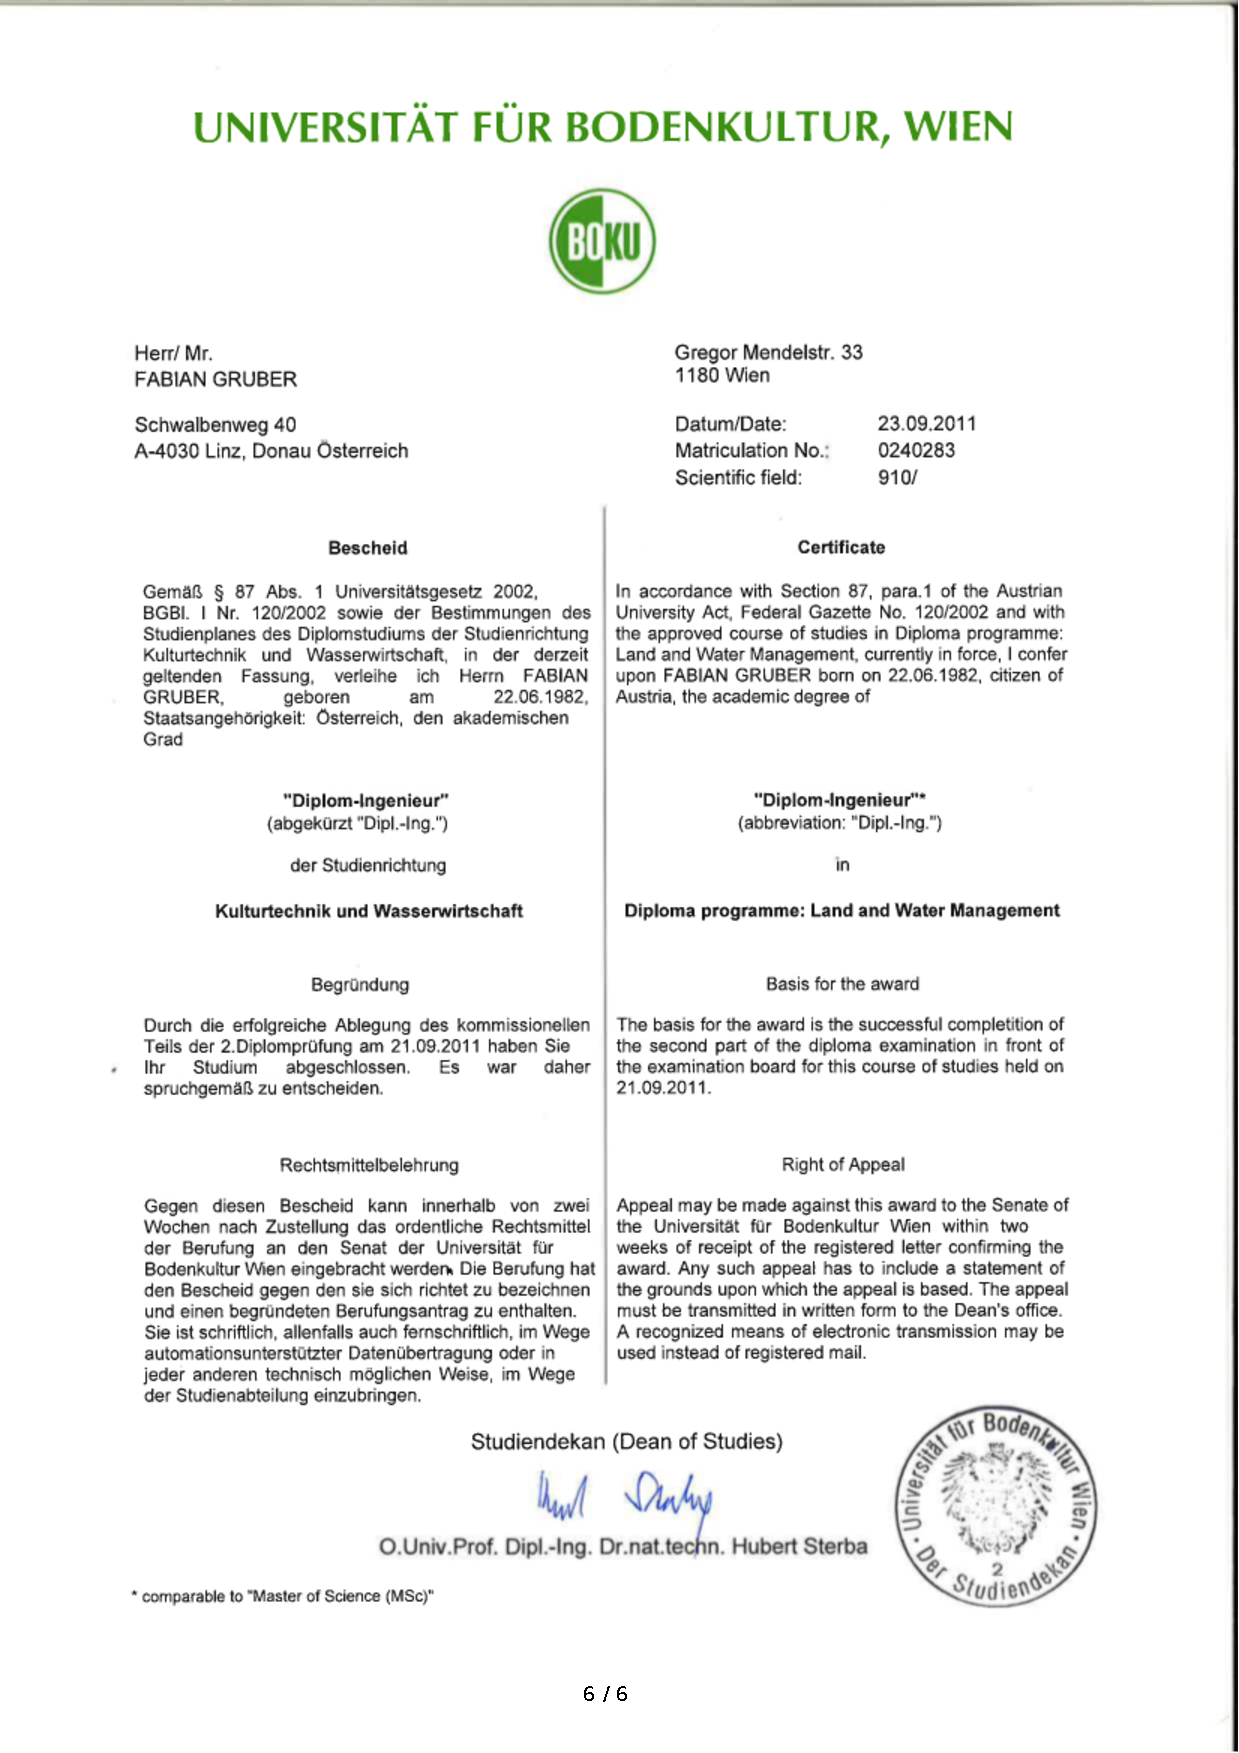
\includepdf{Dipling_seite6von6.pdf}

\end{document}


%% end of file `template.tex'.
